\section{Triển khai Hệ thống}

Sau khi đã phân tích bài toán và thiết kế lời giải qua các chương trước,
chương này trình bày cách BeVietnam được \textbf{triển khai} thành một
hệ thống chạy được. Mục tiêu không phải liệt kê toàn bộ mã nguồn, mà là
làm rõ kiến trúc tổng thể, vai trò của từng dịch vụ và cách ba tính năng
trọng tâm --- bản đồ thời gian thực, Mission Path và xác minh ảnh bằng
thị giác --- được nối với nhau qua các thuật toán cụ thể.

\subsection{Kiến Trúc Tổng Thể}
\contrib

Hệ thống được tổ chức thành một \textit{monorepo} gồm năm thành phần
triển khai độc lập nhưng phối hợp chặt với nhau. Bảng~\ref{tab:impl_services}
tóm tắt vai trò và công nghệ của từng thành phần, còn
Hình~\ref{fig:impl_architecture} mô tả luồng dữ liệu giữa chúng.

\begin{table}[H]
\centering
\caption{Các thành phần triển khai của BeVietnam}
\label{tab:impl_services}
\begin{tabularx}{\textwidth}{>{\raggedright\arraybackslash}p{2.7cm} >{\raggedright\arraybackslash}p{3.3cm} X}
\toprule
\textbf{Thành phần} & \textbf{Công nghệ} & \textbf{Vai trò chính} \\
\midrule
\textbf{Web client} & Next.js (App Router), TypeScript & Feed, Explore (bubble map), Mission Path storyline, capture qua trình duyệt. \\
\textbf{Mobile client} & Android, Jetpack Compose & Trải nghiệm bản đồ thời gian thực, định vị GPS, chụp ảnh thực địa. \\
\textbf{Backend} & FastAPI (async), PostgreSQL, MinIO & Giữ product state, proxy dịch vụ ngoài, xác thực JWT, điều phối xác minh capture. \\
\textbf{AI Core} & FastAPI, các agent, langgraph & Sinh question pool (offline), giải thích đề xuất, và \textbf{Capture Judge} thị giác (runtime). \\
\textbf{vLLM hosting} & vLLM, Qwen2.5-VL-7B, 1$\times$ GPU L40 & Phục vụ mô hình thị giác cho việc chấm điểm ảnh minh chứng. \\
\bottomrule
\end{tabularx}
\end{table}

\begin{figure}[H]
\centering
\resizebox{\textwidth}{!}{%
\begin{tikzpicture}[
    >=Stealth,
    client/.style={draw=primaryblue, fill=blue!4!white, rounded corners=4pt, minimum width=2.6cm, minimum height=0.95cm, align=center, font=\small},
    core/.style={draw=accentblue, fill=accentblue!8!white, rounded corners=5pt, minimum width=3.0cm, minimum height=1.05cm, align=center, font=\small},
    ai/.style={draw=jade, fill=green!5!white, rounded corners=5pt, minimum width=3.0cm, minimum height=1.05cm, align=center, font=\small},
    ext/.style={draw=warnorange, fill=orange!8!white, rounded corners=4pt, minimum width=2.7cm, minimum height=0.9cm, align=center, font=\scriptsize},
    store/.style={draw=darkgray, fill=lightgray, rounded corners=4pt, minimum width=2.7cm, minimum height=0.9cm, align=center, font=\scriptsize}
]
\node[client] (web) at (0,1.2) {Web client\\Next.js};
\node[client] (mob) at (0,-1.2) {Mobile client\\Compose};

\node[core] (be) at (4.3,0) {Backend\\FastAPI};
\node[store] (pg) at (4.3,-2.4) {PostgreSQL\\+ MinIO};

\node[ai] (aicore) at (9.0,0.9) {AI Core\\Capture Judge};
\node[core] (vllm) at (13.3,0.9) {vLLM\\Qwen2.5-VL};

\node[ext] (fsq) at (9.0,-1.4) {Foursquare};
\node[ext] (ow) at (9.0,-2.6) {OpenWeather};
\node[ext] (serp) at (13.3,-0.4) {SerpAPI};

\draw[->, thick, primaryblue] (web) -- (be);
\draw[->, thick, primaryblue] (mob) -- (be);
\draw[->, thick, darkgray] (be) -- (pg);
\draw[->, thick, jade] (be) -- node[above, font=\scriptsize]{verify-capture} (aicore);
\draw[->, thick, accentblue] (aicore) -- node[above, font=\scriptsize]{ảnh + rubric} (vllm);
\draw[->, thick, warnorange] (be) -- node[right, font=\scriptsize, pos=0.55]{nearby} (fsq);
\draw[->, thick, warnorange] (be) -- node[right, font=\scriptsize, pos=0.7]{weather} (ow);
\draw[->, thick, warnorange] (aicore) -- node[right, font=\scriptsize, pos=0.5]{ảnh tham chiếu} (serp);
\end{tikzpicture}}
\caption{Kiến trúc triển khai BeVietnam. Hai client gọi vào backend; backend giữ product state (PostgreSQL/MinIO) và proxy các dịch vụ ngoài (Foursquare, OpenWeather). Riêng việc xác minh ảnh được backend chuyển tiếp cho AI Core, nơi mô hình thị giác Qwen2.5-VL (tự host trên vLLM) thực hiện chấm điểm; ảnh tham chiếu được lấy qua SerpAPI và lưu cache.}
\label{fig:impl_architecture}
\end{figure}

Để minh họa kết quả triển khai thực tế của kiến trúc trên,
Hình~\ref{fig:homepage} là trang chủ của web client (Next.js) đang chạy.

\begin{figure}[H]
\centering
\IfFileExists{images/bevietnam_homepage.jpg}
  {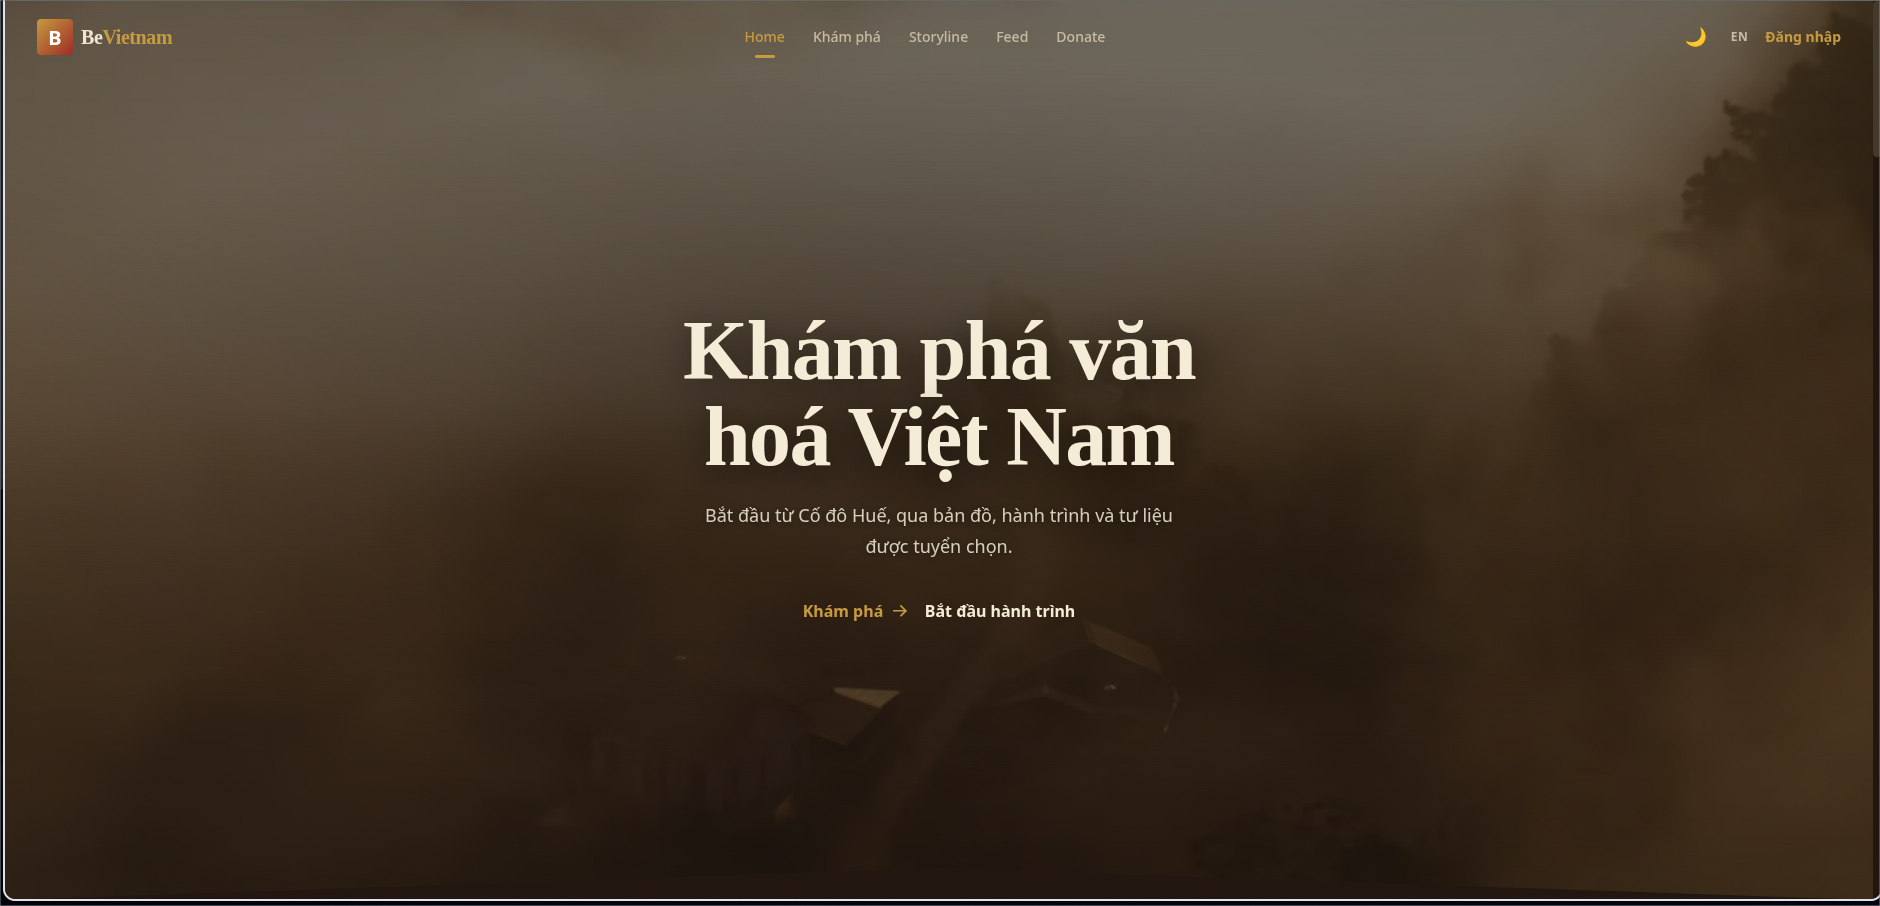
\includegraphics[width=0.85\textwidth]{images/bevietnam_homepage.jpg}}
  {\fbox{\parbox[c][5cm][c]{0.85\textwidth}{\centering\itshape\color{darkgray}images/bevietnam\_homepage.jpg\\(ảnh sẽ được bổ sung)}}}
\caption{Trang chủ web client BeVietnam (Next.js) trong giai đoạn pilot.}
\label{fig:homepage}
\end{figure}

Bên cạnh web, client mobile (Android, Jetpack Compose) cung cấp trải nghiệm
bản đồ thời gian thực, định vị GPS và chụp ảnh thực địa.
Hình~\ref{fig:mobile} là một số màn hình chính của ứng dụng mobile.

\begin{figure}[H]
\centering
\newcommand{\mobtile}[2]{\IfFileExists{#1}{\includegraphics[height=4.6cm]{#1}}{\fbox{\parbox[c][4.6cm][c]{2.4cm}{\centering\scriptsize\itshape\color{darkgray}#2}}}}
\mobtile{images/mobile_login.jpg}{login}\hfill
\mobtile{images/mobile_map.jpg}{map}\hfill
\mobtile{images/mobile_storyline.jpg}{storyline}\hfill
\mobtile{images/mobile_post.jpg}{post}
\caption{Các màn hình chính của client mobile (Android): đăng nhập, bản đồ
thời gian thực, storyline và feed bài viết.}
\label{fig:mobile}
\end{figure}

Một nguyên tắc xuyên suốt là \textbf{backend giữ quyền kiểm soát},
còn các dịch vụ ngoài và AI chỉ là nguồn dữ liệu hoặc bộ suy luận
được gọi khi cần. API của các dịch vụ trả phí (Foursquare, OpenWeather,
Goong) đều được giữ ở server và đi qua một lớp \textit{rate limiter}
chung để bảo vệ hạn mức free-tier trong giai đoạn demo.

\subsection{Pipeline Sinh Tri thức Offline và vLLM Hosting}
\contrib

Một phần lớn giá trị của BeVietnam nằm ở \textbf{nội dung văn hóa} (knowledge
chunk, question pool, spotlight post). Như đã nêu ở các chương trước, nhóm
chủ động \textbf{không} sinh các nội dung này tại runtime mà dựng sẵn
\textit{offline} bằng một pipeline agent riêng, để runtime chỉ việc nạp ra
dữ liệu ổn định. Pipeline này dùng một mô hình ngôn ngữ \textbf{tự host trên
vLLM} (Qwen2.5-Instruct, cùng máy chủ L40 ở Thundercompute, lộ ra qua
cloudflared tại \texttt{api.iamphuckhang.dev}). Lý do tự host là để thay nhà
cung cấp Gemini vốn bị chặn hạn mức (\texttt{429 RESOURCE\_EXHAUSTED}) trong
giai đoạn ingest khối lượng lớn~\cite{vllm_docs}.

\begin{figure}[H]
\centering
\resizebox{\textwidth}{!}{%
\begin{tikzpicture}[
    >=Stealth, node distance=6mm,
    src/.style={draw=darkgray, fill=lightgray, rounded corners=3pt, minimum height=0.8cm, minimum width=2.0cm, align=center, font=\scriptsize},
    proc/.style={draw=accentblue, fill=accentblue!8!white, rounded corners=4pt, minimum height=0.85cm, minimum width=2.3cm, align=center, font=\scriptsize},
    ai/.style={draw=jade, fill=green!6!white, rounded corners=4pt, minimum height=0.85cm, minimum width=2.2cm, align=center, font=\scriptsize},
    out/.style={draw=primaryblue, fill=blue!5!white, rounded corners=4pt, minimum height=0.85cm, minimum width=2.5cm, align=center, font=\scriptsize}
]
\node[src] (books) {Sách OCR\\(.md)};
\node[proc, right=of books] (chunk) {Section-aware\\chunker};
\node[ai, right=of chunk] (vllm) {vLLM LLM\\(grounded\\JSON)};
\node[out, right=of vllm, yshift=8mm] (chunks) {hue\_book\_chunks};
\node[out, right=of vllm, yshift=-8mm] (qp) {question\_pool\\+ hue\_spotlights};
\node[proc, below=10mm of vllm] (review) {Human review\\needs\_review $\to$ approved};
\node[out, right=of review] (seed) {Seed Qdrant /\\backend};
\draw[->, thick, darkgray] (books) -- (chunk);
\draw[->, thick, accentblue] (chunk) -- (vllm);
\draw[->, thick, jade] (vllm) -- (chunks);
\draw[->, thick, jade] (vllm) -- node[below, font=\scriptsize, pos=0.6]{per-landmark} (qp);
\draw[->, thick, darkgray] (chunks) |- (review);
\draw[->, thick, darkgray] (qp) |- (review);
\draw[->, thick, primaryblue] (review) -- (seed);
\end{tikzpicture}}
\caption{Pipeline sinh tri thức offline. Sách OCR được cắt theo mục, mô hình
ngôn ngữ tự host trên vLLM chắt lọc mỗi đoạn thành một dữ kiện văn hóa có dẫn
nguồn; per-landmark sinh question pool và spotlight. Mọi bản ghi mang
\texttt{review\_status = needs\_review} cho tới khi người duyệt.}
\label{fig:offline_pipeline}
\end{figure}

Bảng~\ref{tab:offline_agents} liệt kê các script và agent chính của pipeline.
Hai ràng buộc được giữ xuyên suốt: mọi nội dung phải \textbf{có dẫn nguồn}
(\texttt{source\_text}/\texttt{page\_or\_section} trỏ về một đoạn thật trong
sách) và mặc định \texttt{review\_status = needs\_review} --- tức nội dung do
mô hình sinh không được tin ngay mà phải qua người duyệt mới lên
\texttt{approved}. Khi mô hình lỗi, các agent dùng \textit{fallback} có dẫn
nguồn để dữ liệu không bao giờ rỗng.

\begin{table}[H]
\centering
\caption{Các thành phần của pipeline sinh tri thức offline}
\label{tab:offline_agents}
\begin{tabularx}{\textwidth}{>{\raggedright\arraybackslash}p{4.0cm} >{\raggedright\arraybackslash}p{3.6cm} X}
\toprule
\textbf{Script / Agent} & \textbf{Đầu ra} & \textbf{Vai trò} \\
\midrule
\texttt{ingest\_books.py} & \texttt{hue\_book\_chunks.json} & Cắt sách theo mục + gọi vLLM chắt lọc mỗi chunk thành một KnowledgeChunk có dẫn nguồn. \\
\texttt{generate\_hue\_quests.py} & \texttt{question\_pool.json}, \texttt{hue\_spotlights.json} & Lấy đoạn theo từng địa danh, sinh chuỗi quest + spotlight grounded. \\
\textbf{Question Pool Maker} & câu hỏi/nhiệm vụ có cấu trúc & Biến dữ kiện văn hóa thành ứng viên nhiệm vụ tái sử dụng được. \\
\textbf{Spotlight Maker} & feed post + tag điều kiện & Soạn post grounded, gắn tag weather/time/season. \\
\textbf{Culture Scout} & dữ kiện văn hóa truy hồi & Cung cấp fact có nguồn cho các agent soạn nội dung. \\
\textbf{Safety Keeper} / \texttt{validate\_knowledge\_chunks.py} & dữ liệu đã kiểm & Kiểm schema và an toàn nội dung trước khi seed. \\
\bottomrule
\end{tabularx}
\end{table}

Như vậy, cùng một hạ tầng vLLM trên L40 phục vụ hai vai trò tách biệt: ở
\textit{offline} là mô hình ngôn ngữ sinh nội dung văn hóa, còn ở
\textit{runtime} là mô hình thị giác Qwen2.5-VL chấm ảnh minh chứng. Việc đẩy
toàn bộ sinh nội dung về offline giúp runtime nhẹ, ổn định và không phụ thuộc
hạn mức gọi mô hình theo từng lượt người dùng.

\subsection{Kiến Trúc theo Mô Hình C4}
\contrib

Để mô tả kiến trúc một cách có hệ thống, nhóm dùng \textbf{mô hình C4},
trong đó hệ thống được nhìn ở nhiều mức trừu tượng khác nhau: từ mức
\textit{bối cảnh} trừu tượng nhất cho tới mức \textit{thành phần} chi tiết
bên trong từng phía. Phần này trình bày bốn lớp: một lớp trừu tượng tổng
quan, rồi ba lớp chi tiết lần lượt cho frontend, backend và AI service.

\subsubsection{Abstract Layer}
\contrib

Ở mức trừu tượng nhất (Hình~\ref{fig:c4_context}), toàn bộ hệ thống được
xem như một hộp duy nhất: du khách tương tác với BeVietnam, còn BeVietnam
gọi tới một số dịch vụ ngoài để lấy POI, thời tiết, ảnh tham chiếu và
bản đồ nền.

\begin{figure}[H]
\centering
\resizebox{0.92\textwidth}{!}{%
\begin{tikzpicture}[
    >=Stealth,
    person/.style={draw=primaryblue, fill=primaryblue, text=white, rounded corners=3pt, minimum width=2.4cm, minimum height=1.1cm, align=center, font=\small},
    system/.style={draw=primaryblue, fill=accentblue!18!white, rounded corners=5pt, minimum width=3.6cm, minimum height=1.5cm, align=center, font=\small},
    ext/.style={draw=darkgray, fill=lightgray, rounded corners=4pt, minimum width=2.5cm, minimum height=0.9cm, align=center, font=\scriptsize},
    rel/.style={->, thick, darkgray, font=\scriptsize}
]
\node[person] (u) at (0,0) {\textbf{Du khách}\\{\scriptsize[Person]}};
\node[system] (sys) at (5,0) {\textbf{Hệ thống BeVietnam}\\{\scriptsize[Software System]}\\{\scriptsize Khám phá, gợi ý, storyline}};
\node[ext] (fsq)  at (10,1.8) {Foursquare};
\node[ext] (ow)   at (10,0.6) {OpenWeather};
\node[ext] (serp) at (10,-0.6) {SerpApi};
\node[ext] (goong)at (10,-1.8) {Goong Maps};
\draw[rel] (u) -- node[above]{dùng web/mobile} (sys);
\draw[rel] (sys) -- (fsq);  \draw[rel] (sys) -- (ow);
\draw[rel] (sys) -- (serp); \draw[rel] (sys) -- (goong);
\end{tikzpicture}}
\caption{Du khách dùng BeVietnam; hệ thống lấy dữ liệu từ bốn dịch vụ ngoài.}
\label{fig:c4_context}
\end{figure}

\subsubsection{Frontend Layer}
\contrib

Mở hộp ``client'' ra, ta có hai container giao diện dùng chung một backend
(Hình~\ref{fig:c4_frontend}). Web và mobile có cấu trúc tương tự: một lớp
màn hình/tính năng, một lớp gọi API, và (ở mobile) một lớp ViewModel +
repository theo kiến trúc luồng dữ liệu một chiều.

\begin{figure}[H]
\centering
\resizebox{\textwidth}{!}{%
\begin{tikzpicture}[
    >=Stealth,
    comp/.style={draw=accentblue, fill=accentblue!8!white, rounded corners=4pt, minimum width=3.0cm, minimum height=0.95cm, align=center, font=\scriptsize},
    ext/.style={draw=darkgray, fill=lightgray, rounded corners=4pt, minimum width=2.6cm, minimum height=0.9cm, align=center, font=\scriptsize},
    rel/.style={->, thick, darkgray}
]
% Web container
\node[comp] (wpage) at (0,1.4) {\textbf{Feature Pages}\\{\scriptsize Explore, Storyline, Feed}};
\node[comp] (wapi)  at (0,0)   {\textbf{API Client}\\{\scriptsize lib/api.ts}};
\node[comp] (wi18n) at (0,-1.4){\textbf{i18n + UI}\\{\scriptsize translations}};
\begin{scope}[on background layer]
\node[draw=primaryblue, thick, dashed, rounded corners=6pt, fit=(wpage)(wapi)(wi18n), inner sep=8pt, label={[font=\scriptsize\bfseries,primaryblue]above:Web [Next.js]}] (webbox) {};
\end{scope}
% Mobile container
\node[comp] (mscr) at (5.6,1.4) {\textbf{Screens}\\{\scriptsize ExploreScreen}};
\node[comp] (mvm)  at (5.6,0)   {\textbf{ViewModel}\\{\scriptsize ExploreViewModel}};
\node[comp] (mrepo)at (5.6,-1.4){\textbf{Repository + Retrofit}\\{\scriptsize BeVietnamApi, DTO/Mapper}};
\begin{scope}[on background layer]
\node[draw=primaryblue, thick, dashed, rounded corners=6pt, fit=(mscr)(mvm)(mrepo), inner sep=8pt, label={[font=\scriptsize\bfseries,primaryblue]above:Mobile [Compose]}] (mobbox) {};
\end{scope}
\node[ext] (be) at (11,0) {\textbf{Backend API}\\{\scriptsize [FastAPI]}};
\draw[rel] (wpage) -- (wapi); \draw[rel] (wapi) -- (wi18n);
\draw[rel] (mscr) -- (mvm); \draw[rel] (mvm) -- (mrepo);
\draw[rel] (wapi.east) -- node[above,font=\scriptsize]{HTTPS/JSON} (be.west);
\draw[rel] (mrepo.east) -- (be.west);
\end{tikzpicture}}
\caption{C4 mức container/thành phần — phía frontend. Web (Next.js) và mobile (Compose) chia sẻ cùng một backend qua HTTPS/JSON.}
\label{fig:c4_frontend}
\end{figure}

\subsubsection{Backend Layer}
\contrib

Bên trong container backend (Hình~\ref{fig:c4_backend}), các thành phần
được xếp theo tầng: lớp \textit{endpoint} nhận request, gọi xuống lớp
\textit{service} (nghiệp vụ và proxy dịch vụ ngoài) và lớp \textit{repository}
(đọc/ghi dữ liệu). Các thành phần xuyên suốt như rate limiter, xác thực
JWT và AI Core Client phục vụ cho nhiều endpoint.

\begin{figure}[H]
\centering
\resizebox{\textwidth}{!}{%
\begin{tikzpicture}[
    >=Stealth,
    comp/.style={draw=accentblue, fill=accentblue!8!white, rounded corners=4pt, minimum width=3.1cm, minimum height=0.95cm, align=center, font=\scriptsize},
    ext/.style={draw=darkgray, fill=lightgray, rounded corners=4pt, minimum width=2.4cm, minimum height=0.85cm, align=center, font=\scriptsize},
    rel/.style={->, thick, darkgray}
]
\node[comp] (ep)   at (0,1.6)  {\textbf{API Endpoints}\\{\scriptsize places, feed, storyline, auth}};
\node[comp] (svc)  at (0,0)    {\textbf{Service Layer}\\{\scriptsize foursquare, weather, post, pool}};
\node[comp] (repo) at (0,-1.6) {\textbf{Repository + Models}\\{\scriptsize Place, User, Pref, Capture}};
\node[comp] (rl)   at (4.3,0.6)  {\textbf{Rate Limiter}};
\node[comp] (jwt)  at (4.3,-0.6) {\textbf{JWT Auth}};
\node[comp] (aicli)at (4.3,1.8)  {\textbf{AI Core Client}};
\begin{scope}[on background layer]
\node[draw=primaryblue, thick, dashed, rounded corners=6pt, fit=(ep)(repo)(aicli)(jwt), inner sep=9pt, label={[font=\scriptsize\bfseries,primaryblue]above:Backend [FastAPI]}] (bebox) {};
\end{scope}
\node[ext] (pg)    at (0,-3.4) {PostgreSQL};
\node[ext] (minio) at (2.6,-3.4) {MinIO};
\node[ext] (api3)  at (9,0)   {\textbf{Foursquare}\\\textbf{OpenWeather}\\{\scriptsize [Third-party]}};
\node[ext] (aicore)at (9,2.0)  {\textbf{AI Core}\\{\scriptsize [FastAPI]}};
\draw[rel] (ep) -- (svc); \draw[rel] (svc) -- (repo);
\draw[rel] (repo) -- (pg); \draw[rel] (repo) -- (minio);
\draw[rel] (svc) -- (rl); \draw[rel] (rl) -- (api3);
\draw[rel] (ep) -- (jwt);
\draw[rel] (ep) -- (aicli); \draw[rel] (aicli) -- (aicore);
\end{tikzpicture}}
\caption{C4 mức thành phần — phía backend. Endpoint $\to$ service $\to$ repository; rate limiter chắn các lời gọi dịch vụ ngoài; AI Core Client chuyển tiếp việc xác minh ảnh.}
\label{fig:c4_backend}
\end{figure}

\subsubsection{AI Service}
\contrib

Cuối cùng, mở container AI Core (Hình~\ref{fig:c4_ai}). Phần nội dung
(question pool, bài viết) do các agent sinh offline, còn ở runtime chỉ
agent \textbf{Capture Judge} hoạt động: nó lấy ảnh tham chiếu rồi gọi mô
hình thị giác qua một LLM Gateway thống nhất.

\begin{figure}[H]
\centering
\resizebox{\textwidth}{!}{%
\begin{tikzpicture}[
    >=Stealth,
    comp/.style={draw=jade, fill=green!6!white, rounded corners=4pt, minimum width=3.1cm, minimum height=0.95cm, align=center, font=\scriptsize},
    ext/.style={draw=darkgray, fill=lightgray, rounded corners=4pt, minimum width=2.5cm, minimum height=0.85cm, align=center, font=\scriptsize},
    rel/.style={->, thick, darkgray}
]
\node[comp] (routes) at (0,1.6)  {\textbf{API Routes}\\{\scriptsize verify-capture, generate-*}};
\node[comp] (judge)  at (0,0)    {\textbf{Capture Judge}\\{\scriptsize runtime, thị giác}};
\node[comp] (offline)at (0,-1.6) {\textbf{Offline Agents}\\{\scriptsize Pool Maker, Trip Advisor, Spotlight}};
\node[comp] (ref)    at (4.3,1.0)  {\textbf{Reference Fetcher}\\{\scriptsize SerpApi + cache}};
\node[comp] (gw)     at (4.3,-0.6) {\textbf{LLM Gateway}\\{\scriptsize VLLMGateway}};
\begin{scope}[on background layer]
\node[draw=jade, thick, dashed, rounded corners=6pt, fit=(routes)(offline)(ref)(gw), inner sep=9pt, label={[font=\scriptsize\bfseries,jade]above:AI Core [FastAPI]}] (aibox) {};
\end{scope}
\node[ext] (vllm) at (9,-0.6) {\textbf{vLLM}\\{\scriptsize Qwen2.5-VL}};
\node[ext] (serp) at (9,1.0)  {\textbf{SerpApi}};
\draw[rel] (routes) -- (judge); \draw[rel] (routes) -- (offline);
\draw[rel] (judge) -- (ref); \draw[rel] (ref) -- (serp);
\draw[rel] (judge) -- (gw); \draw[rel] (gw) -- (vllm);
\end{tikzpicture}}
\caption{C4 mức thành phần — AI service. Capture Judge là agent runtime duy nhất, dùng Reference Fetcher (SerpApi + cache) và LLM Gateway tới mô hình thị giác vLLM.}
\label{fig:c4_ai}
\end{figure}

\subsection{Lớp Dữ Liệu và API}
\contrib

Bốn thực thể trừu tượng ở Chương Abstraction được hiện thực thành các
bảng và endpoint cụ thể (Bảng~\ref{tab:impl_endpoints}). Backend dùng
PostgreSQL cho dữ liệu có cấu trúc (POI, người dùng, tuỳ chọn cá nhân,
capture) và MinIO cho ảnh.

\begin{table}[H]
\centering
\caption{Một số endpoint chính của backend}
\label{tab:impl_endpoints}
\begin{tabularx}{\textwidth}{>{\ttfamily\small\raggedright\arraybackslash}p{4.7cm} X}
\toprule
\textbf{\normalfont Endpoint} & \textbf{Vai trò} \\
\midrule
GET /places/nearby & POI thời gian thực quanh một tọa độ (proxy Foursquare). \\
GET /weather & Thời tiết khu vực: nhiệt độ, UV ước lượng, lượng mưa. \\
GET /question-pool & Toàn bộ kho nhiệm vụ cho Mission Path. \\
GET /feed & Feed gợi ý đã cá nhân hóa theo tuỳ chọn người dùng. \\
POST /storyline/verify-capture & Chuyển ảnh minh chứng sang AI Core để chấm điểm. \\
GET/PUT /me/preferences & Đọc/ghi tuỳ chọn cá nhân phục vụ xếp hạng feed. \\
\bottomrule
\end{tabularx}
\end{table}

\subsection{Realtime Bubble Map}
\contrib

Khi khảo sát các ứng dụng bản đồ và review, nhóm nhận thấy người dùng
phải mở nhiều nguồn khác nhau để xem địa điểm, thời tiết và mô tả. Vì
vậy, trong bản pilot tại Huế, nhóm chọn cách gom các thông tin cần thiết
về một endpoint để client chỉ cần gọi một lần khi mở màn hình Explore.

Bản đồ thời gian thực neo vào vị trí GPS thực của người dùng. Khi vào màn
hình, client xin quyền và lấy tọa độ hiện tại, sau đó gọi
\texttt{/places/nearby} với bán kính cố định 3km, được backend lấy từ
Foursquare Places API~\cite{foursquare_places}. Mỗi POI trả về được
client vẽ thành một bong bóng, với bán kính co giãn theo khoảng cách
\textit{haversine}~\cite{sinnott1984} tới người dùng: càng gần thì bong
bóng càng lớn. Pseudocode~\ref{lst:bubble} mô tả bước dựng bong bóng.

\begin{lstlisting}[caption={Dựng bong bóng theo khoảng cách tới người dùng}, label={lst:bubble}]
INPUT  places[], user_gps
maxDist = max( haversine(user_gps, p.coord) for p in places )
FOR each p in places:
    d        = haversine(user_gps, p.coord)
    weight   = 1 - d / maxDist          # 1 = gan nhat, 0 = xa nhat
    radius   = BASE + weight * SPREAD    # px
    color    = colorOfCategory(p.bucket) # food/lodging/culture/...
    emit bubble(center = p.coord, radius, color, label = p.name)
\end{lstlisting}

Toàn bộ POI là dữ liệu sống của Foursquare nên không cố định theo địa
phương; ứng dụng hoạt động ở bất kỳ đâu người dùng đứng. Một chip thời
tiết của khu vực (nhiệt độ, UV, mưa) lấy từ OpenWeather
API~\cite{openweather_api} được hiển thị kèm để bổ sung ngữ cảnh ra
quyết định.

\subsection{Storyline Mission Path}
\contrib

Mission Path nạp toàn bộ kho nhiệm vụ từ \texttt{/question-pool} rồi dựng
một lộ trình dạng các nút uốn lượn. Trạng thái của mỗi nút được suy ra
hoàn toàn từ tập nhiệm vụ đã hoàn thành (lưu cục bộ), theo luật mở khóa
tuần tự ở Pseudocode~\ref{lst:unlock}.

\begin{lstlisting}[caption={Luật trạng thái nút trên Mission Path}, label={lst:unlock}]
INPUT  tasks[], completedIds
activeIndex = first index i where tasks[i].id not in completedIds
FOR each task[i]:
    IF task[i].id in completedIds:  state = DONE      # da hoan thanh
    ELIF i == activeIndex:          state = ACTIVE    # dang mo, co the lam
    ELSE:                           state = LOCKED    # chua mo khoa
\end{lstlisting}

Khi người dùng chạm vào một nút đang mở, hệ thống hiển thị chi tiết nhiệm
vụ (tiêu đề, yêu cầu, giải nghĩa văn hóa) cùng nút chụp/tải ảnh. Ảnh được
gửi đi xác minh; nếu đạt, nhiệm vụ chuyển sang DONE và nút kế tiếp tự
động trở thành ACTIVE.

\subsection{Vision Capture Verification}
\contrib

Đây là tính năng \textbf{duy nhất} bắt buộc dùng mô hình AI tại thời gian
thực. Khi backend nhận ảnh và chuyển sang AI Core, agent \textbf{Capture
Judge} thực hiện một pipeline bốn bước
(Hình~\ref{fig:impl_capture}): giải mã ảnh người dùng, lấy ảnh tham chiếu
của chủ thể nhiệm vụ (tìm qua SerpApi Google Images~\cite{serpapi} rồi
lưu cache theo từng nhiệm vụ), yêu cầu mô hình thị giác chấm điểm theo
rubric, và ánh xạ điểm sang trạng thái cuối cùng.

\begin{figure}[H]
\centering
\resizebox{\textwidth}{!}{%
\begin{tikzpicture}[
    >=Stealth,
    pstep/.style={draw=jade, fill=green!5!white, rounded corners=4pt, minimum width=3.0cm, minimum height=1.0cm, align=center, font=\small},
    dec/.style={draw=warnorange, fill=orange!8!white, rounded corners=4pt, minimum width=2.6cm, minimum height=0.9cm, align=center, font=\scriptsize}
]
\node[pstep] (c1) at (0,0) {Giải mã ảnh\\người dùng};
\node[pstep] (c2) at (3.7,0) {Lấy ảnh tham chiếu\\(SerpAPI + cache)};
\node[pstep] (c3) at (7.6,0) {Mô hình thị giác\\chấm điểm rubric};
\node[pstep] (c4) at (11.4,0) {Ánh xạ ngưỡng\\$\to$ trạng thái};

\draw[->, thick, jade] (c1) -- (c2);
\draw[->, thick, jade] (c2) -- (c3);
\draw[->, thick, jade] (c3) -- (c4);

\node[dec] (a) at (11.4,-1.9) {approved\\/ needs\_review\\/ rejected};
\draw[->, thick, warnorange] (c4) -- (a);
\end{tikzpicture}}
\caption{Pipeline xác minh ảnh của Capture Judge. Nếu không tìm được ảnh tham chiếu, mô hình vẫn chấm dựa trên mô tả nhiệm vụ; nếu mô hình không sẵn sàng, hệ thống trả \textit{needs\_review} thay vì tự ý chấp nhận.}
\label{fig:impl_capture}
\end{figure}

Rubric chấm điểm được đưa thẳng vào system prompt của mô hình để kết quả
mang tính tất định hơn (Bảng~\ref{tab:impl_rubric}). Mô hình nhận hai
ảnh (tham chiếu và của người dùng) cùng mô tả nhiệm vụ, rồi trả về một
JSON gồm điểm, nhãn và lý do.

\begin{table}[H]
\centering
\caption{Rubric chấm điểm độ khớp ảnh (thang 0--1)}
\label{tab:impl_rubric}
\begin{tabularx}{\textwidth}{>{\raggedright\arraybackslash}p{2.2cm} X}
\toprule
\textbf{Khoảng điểm} & \textbf{Diễn giải} \\
\midrule
$0.0 - 0.2$ & Hoàn toàn khác, không liên quan đến chủ thể yêu cầu. \\
$0.2 - 0.4$ & Vẫn khác, chỉ nhỉnh hơn một chút (đúng chủ đề chung nhưng sai đối tượng). \\
$0.4 - 0.6$ & Gần đúng nhưng vẫn sai địa điểm (ví dụ: yêu cầu ``Ngọ Môn'' nhưng ảnh là ``Tử Cấm Thành''). \\
$0.7 - 0.9$ & Ảnh tốt, đúng chủ thể/địa điểm được yêu cầu. \\
$1.0$ & Trùng khớp rõ ràng, không nghi ngờ. \\
\bottomrule
\end{tabularx}
\end{table}

Quy tắc quyết định được phát biểu tường minh trong
Định nghĩa~\ref{def:verify-rule}, với hai ngưỡng $\tau_a = 0.7$ và
$\tau_r = 0.4$ phân tách ba vùng.

\begin{mydef}{Quy Tắc Quyết Định Xác Minh}{verify-rule}
Cho điểm khớp $\sigma \in [0,1]$ do mô hình thị giác trả về (hoặc $\sigma$
không xác định khi mô hình không sẵn sàng), trạng thái xác minh là
\[
\mathrm{status}(\sigma) =
\begin{cases}
\textsf{approved}      & \sigma \ge \tau_a \\
\textsf{needs\_review} & \tau_r \le \sigma < \tau_a \ \text{hoặc}\ \sigma\ \text{không xác định} \\
\textsf{rejected}      & \sigma < \tau_r
\end{cases}
\]
Chỉ trạng thái \textsf{approved} mới mở khóa nút nhiệm vụ kế tiếp.
\end{mydef}

Thuật toán~\ref{alg:capture} trình bày toàn bộ luồng từ ảnh người dùng
tới trạng thái cuối.

\begin{algorithm}[H]
\caption{Ánh xạ điểm rubric sang trạng thái xác minh}
\label{alg:capture}
\begin{algorithmic}[1]
\Require Ảnh người dùng \textit{img}, nhiệm vụ $q$
\State $\textit{ref} \gets \mathrm{getReference}(q.\textit{id},\ \mathrm{subject}(q))$ \Comment{cache hoặc SerpAPI}
\State $\sigma \gets \mathrm{VLM.judge}([\textit{ref}, \textit{img}],\ \text{rubric},\ q)$ \Comment{$\in [0,1]$}
\If{$\sigma$ không xác định} \State \Return \textsf{needs\_review} \EndIf
\If{$\sigma \ge 0.7$} \State \Return \textsf{approved}
\ElsIf{$\sigma \ge 0.4$} \State \Return \textsf{needs\_review}
\Else\ \State \Return \textsf{rejected}
\EndIf
\end{algorithmic}
\end{algorithm}

\begin{myinsight}{Kiểm soát AI bằng cấu trúc}{capture}
Điểm đáng chú ý về tư duy tính toán ở đây là cách AI được ``đóng khung''.
Thay vì hỏi mô hình ``ảnh này có hợp lệ không'' và tin tuyệt đối vào câu
trả lời, hệ thống cung cấp ảnh tham chiếu làm mốc so sánh, ép mô hình
chấm theo một rubric tường minh, và để các \textbf{ngưỡng số} ở phía
backend quyết định trạng thái. Nhờ vậy, một thành phần vốn rất ``mềm''
như suy luận thị giác vẫn được đưa về một pipeline có đầu vào, đầu ra và
quy tắc rõ ràng --- đúng tinh thần biến cái định tính thành cái tính
toán được.
\end{myinsight}

\begin{note}[Hạn chế hiện tại]
Phần xác minh ảnh hiện chỉ phù hợp với các nhiệm vụ có chủ thể quan sát
rõ (một công trình, một chi tiết kiến trúc cụ thể). Với các nhiệm vụ
mang tính cảm nhận văn hóa hoặc hành vi --- ví dụ ``cảm nhận không khí
phiên chợ'' --- mô hình thị giác khó chấm chính xác, nên nhóm vẫn cần
một cơ chế duyệt thủ công (trạng thái \textsf{needs\_review}) cho nhóm
nhiệm vụ đó.
\end{note}

\subsection{Mô Hình AI Tự Host}
\contrib

Trong toàn bộ hệ thống, chỉ có \textbf{một} tính năng cần mô hình AI ở
thời gian thực là Capture Judge; các nội dung khác (question pool, bài
viết feed) được sinh trước offline. Vì việc xác minh ảnh là bài toán thị
giác, nhóm chọn một mô hình ngôn ngữ-thị giác (VLM) là
\textbf{Qwen2.5-VL-7B-Instruct}~\cite{qwen25vl} và tự host trên
vLLM~\cite{kwon2023vllm, vllm_docs} với một GPU L40 (48\,GB). Một mô hình
bản 7B ở định dạng bfloat16 chiếm khoảng 16\,GB, còn dư nhiều bộ nhớ cho
KV-cache (cơ chế quản lý bộ nhớ PagedAttention của vLLM~\cite{kwon2023vllm}),
nên một card L40 là đủ để phục vụ tính năng này mà không cần thêm phần cứng. Việc dùng mô hình thị giác cũng cho
phép gửi đồng thời \textit{hai} ảnh (tham chiếu và của người dùng) trong
một lượt suy luận để mô hình so sánh trực tiếp.
